\newpage

Il existe encore de nombreuses difficultés pour expliquer les mécanismes moléculaires responsables de l’évolution de l’expression des gènes. Comme je l’ai précédemment mentionné, l'expression des gènes codant pour des protéines évolue lentement chez les vertébrés \citep{brawand_evolution_2011, necsulea_evolutionary_2014, cardoso-moreira_gene_2019}. Au contraire, les éléments \gls{cis}-régulateurs évoluent plus rapidement, que ce soit au niveau de leurs séquences mais aussi de leurs activités \citep{cheng_principles_2014, villar_enhancer_2015}. Peu d’études ont relié ces deux observations, et celles-ci ont révélé une faible corrélation entre le taux d’évolution de la régulation et le taux d’évolution de l’expression des gènes \citep{wong_interplay_2017, berthelot_complexity_2018}. Une hypothèse avancée met en avant la complexité et la redondance fonctionnelle des paysages \gls{cis}-régulateurs qui pourrait assurer une stabilité de l’expression au cours de l’évolution \citep{osterwalder_enhancer_2018, berthelot_complexity_2018}. Une autre explication pourrait résider dans la difficulté d’associer les éléments \gls{cis}-régulateurs à leurs gènes cibles. Les prédictions par une approche de voisinage des paires gènes-\gls{amplificateur} employées dans ces études pourraient en effet résulter en des associations partiellement erronées et ainsi affecter négativement les tentatives de corrélation entre leurs taux d’évolution. Les mesures expérimentales des paysages \gls{cis}-régulateurs par les contacts de la chromatine centrés sur les promoteurs des gènes (\acrshort{PCHi-C}) pourraient être en mesure de fournir des associations régulatrices plus pertinentes. De telles données s’accumulent aujourd’hui sur des échantillons humains mais également sur la souris, permettant d’effectuer une analyse comparative de ces paysages \gls{cis}-régulateurs.\\

Cette Partie contient le travail publié dans Genome Research au cours duquel je me suis intéressé à analyser conjointement l’évolution des paysages \gls{cis}-régulateurs mesurés par \acrshort{PCHi-C} ainsi que l’évolution de l’expression des gènes. Dans un premier temps, j’ai compilé et homogénéisé l’ensemble des données de \acrshort{PCHi-C} disponibles à l’échelle génomique pour l’humain et la souris. J’ai également réuni plusieurs prédictions d’\glspl{amplificateur} obtenus à partir de différentes méthodes. Ensuite je me suis attaché à décrire plusieurs aspects de l’évolution de ces paysages \gls{cis}-régulateurs. J’ai d’abord analysé la conservation des séquences des régions et des \glspl{amplificateur} contactés par les promoteurs des gènes au sein des génomes de 8 espèces de vertébrés (humain, souris, lapin, chien, éléphant, vache, opossum, poulet). J’ai mesuré la proportion de ces paires gène-\gls{amplificateur} homologues conservées en synténie chez ces mêmes espèces. Entre l’humain et la souris, j’ai évalué la conservation des contacts de chromatine entre les gènes orthologues et les régions contactées homologues avec une attention particulière pour les mesures effectuées sur des types cellulaires similaires. J’ai utilisé des données d’expression des gènes au sein de plusieurs types cellulaires et stades de développement pour évaluer les relations entre l’évolution des paysages \gls{cis}-régulateur et l’évolution de l’expression des gènes chez l’humain et la souris. \\

J’ai dans un premier temps pu confirmer que les données de \acrshort{PCHi-C} sont enrichies en relations régulatrices. Grâce à des analyses évolutives, j’ai ensuite montré que les séquences qui sont contactées par les promoteurs de gènes sont significativement mieux conservées au cours de l'évolution qu’un attendu aléatoire. Cette conservation de séquence augmente avec la distance génomique entre les promoteurs de gènes et les régions contactées. Les paires promoteur-\gls{amplificateur} impliquées dans des contacts de chromatine ont également tendance à être maintenues en synténie au cours de l'évolution des vertébrés. J’ai également montré que les contacts de chromatine entre les promoteurs et les \glspl{amplificateur} sont significativement conservés entre l'homme et la souris. Là encore, l'étendue de la conservation évolutive est plus importante pour des contacts à grandes distances génomiques. Cette observation indique que les contacts promoteur-\gls{amplificateur} à longue distance représentent une partie importante des paysages \gls{cis}-régulateurs, et souligne que la présence de contacts régulateurs impose de fortes contraintes fonctionnelles sur l'évolution du génome. En analysant l’expression des gènes, j’ai pu démontré que les niveaux d'expression et l’étendu de l’expression des gènes sont corrélés positivement avec la complexité des paysages \gls{cis}-régulateurs. Autrement dit, les gènes ayant des niveaux d'expression plus élevés et les gènes actifs dans de nombreux tissus et stades de développement sont en contact avec de nombreux amplificateurs. Enfin, j’ai révélé que l’évolution du patron d’expression des gènes est significativement corrélée avec l'évolution des paysages \gls{cis}-régulateurs. Cette observation est valable pour l’ensemble des comparaisons effectuées, en termes d’évolution des séquences des \glspl{amplificateur} contactés, de rupture de synténie entre promoteurs et \glspl{amplificateur} ainsi que de gains/pertes de contacts de chromatine entre gènes et \glspl{amplificateur} homologues.

\chapter{Article 2 - Long-range promoter-enhancer contacts are conserved during evolution and contribute to gene expression robustness}
\label{chap:chap3}
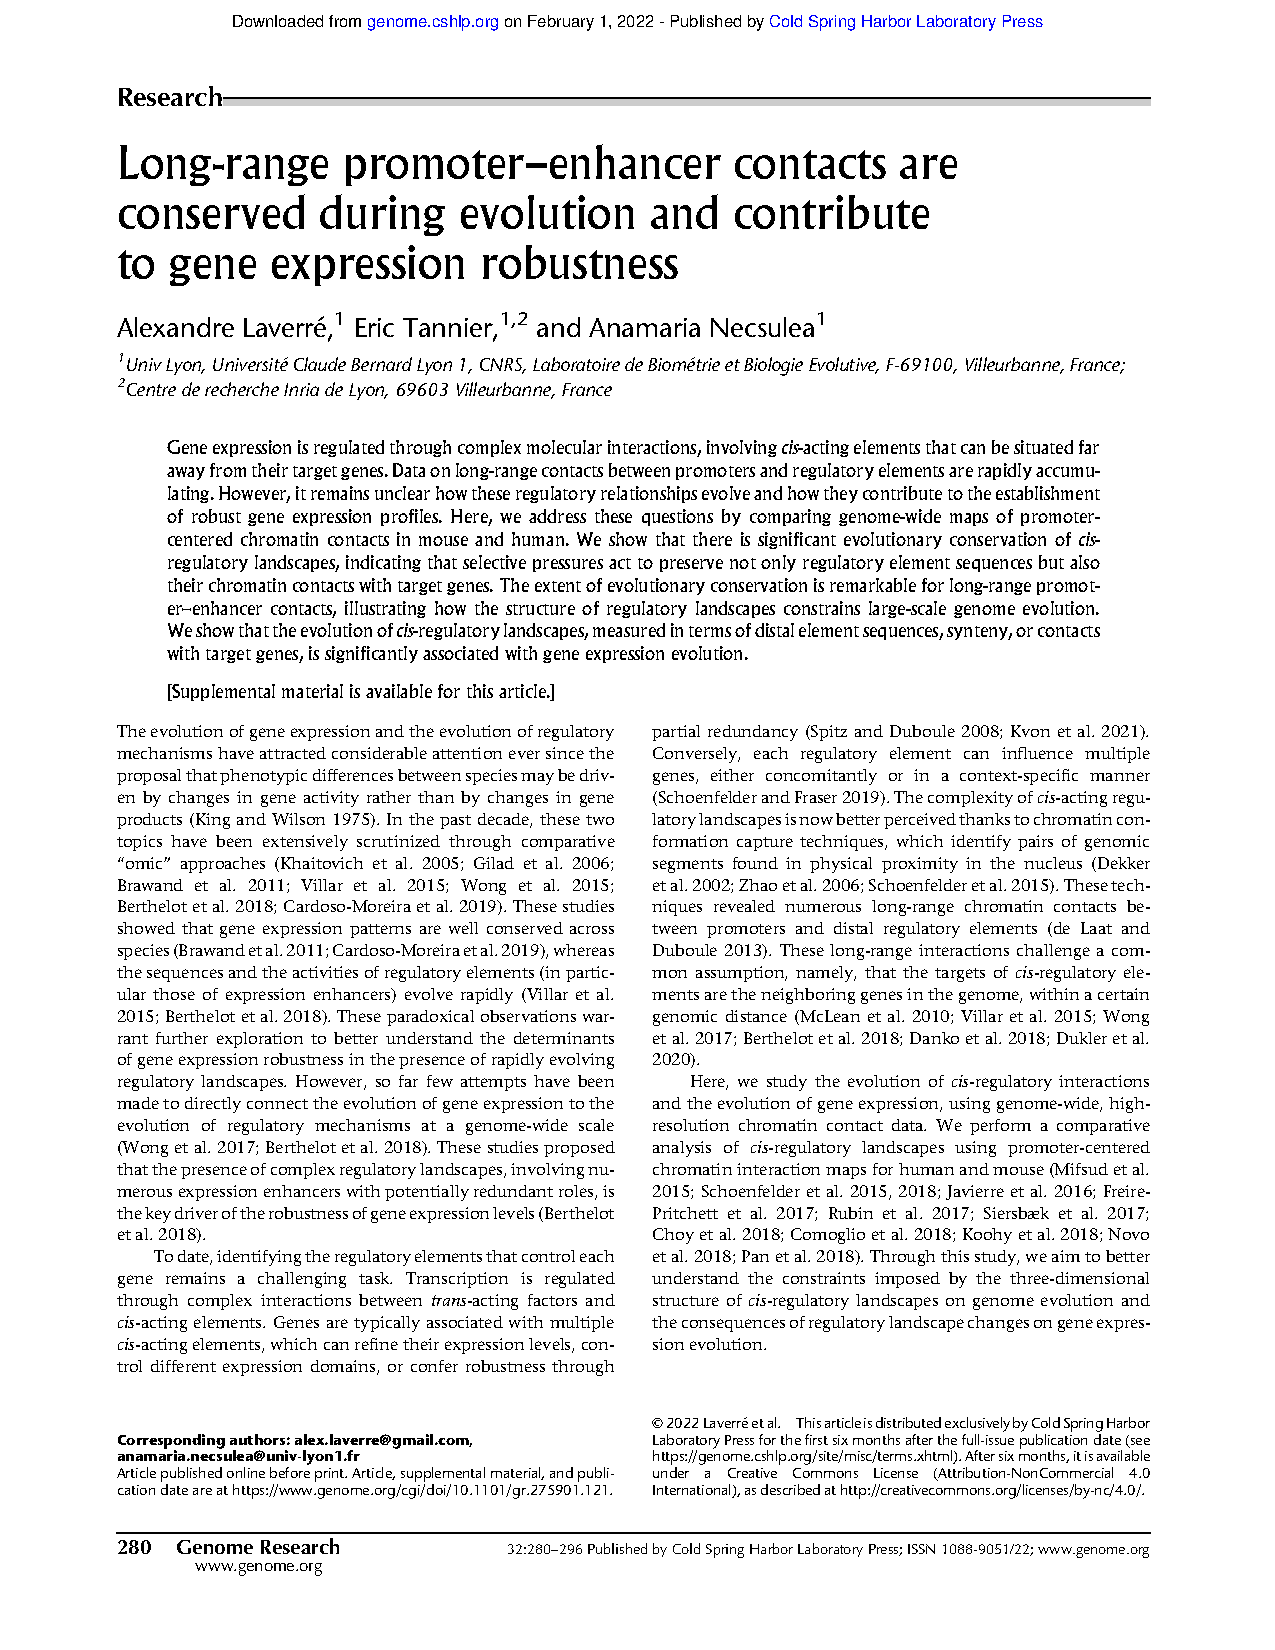
\includepdf[pages=-]{parts/11_Laverre2022.pdf}